%% ===========================================================================
%%  Sensor Identity Does Not Transfer
%%  Elsevier CAS double-column template (cas-dc), as used for the previous
%%  submission.  Compile on Overleaf with pdfLaTeX.
%%
%%  Requires: cas-dc.cls + cas-common.sty (bundled with Overleaf's Elsevier CAS
%%  template).  Figures live in ./figures, TikZ diagrams in ./diagrams.tex.
%%
%%  Every number is produced by a script in ../src and stored in ../results;
%%  the provenance of each table is given in a comment above it.
%% ===========================================================================
\documentclass[a4paper,fleqn]{cas-dc}

\usepackage[numbers]{natbib}
\usepackage{amsmath,amssymb}
\usepackage{booktabs}
\usepackage{graphicx}
\usepackage{multirow}
\usepackage{tikz}
\usetikzlibrary{arrows.meta,positioning,calc,fit}

\graphicspath{{figures/}}

\newcommand{\macf}{macro-F\textsubscript{1}}

% The CAS class prints an "ORCID(s):" line in the first-page footnote block even when
% no ORCID is supplied. Suppress the empty label; delete this if ORCIDs are added.
\makeatletter
\AtBeginDocument{\@ifundefined{printorcid}{}{\renewcommand{\printorcid}{}}}
\makeatother

%% ===========================================================================
%%  TikZ method diagrams, in the style of the previous submission's Figs. 1,3,4,5.
%%  Self-contained: no external image files, so Overleaf compiles them directly.
%% ===========================================================================

\tikzset{
  blk/.style   = {draw, rounded corners=1pt, align=center, font=\scriptsize,
                  minimum height=5.2mm, inner xsep=3pt, fill=white},
  shaded/.style= {blk, fill=black!6},
  hdr/.style   = {blk, fill=black!12, font=\scriptsize\bfseries},
  io/.style    = {blk, fill=black!14, font=\scriptsize\bfseries},
  note/.style  = {align=center, font=\tiny, text=black!65},
  ar/.style    = {-{Latex[length=1.6mm,width=1.2mm]}, thin},
  arb/.style   = {-{Latex[length=1.6mm,width=1.2mm]}, thin, dashed},
}

% ---------------------------------------------------------------- Fig: HAR-MLP
\newcommand{\figMLP}{%
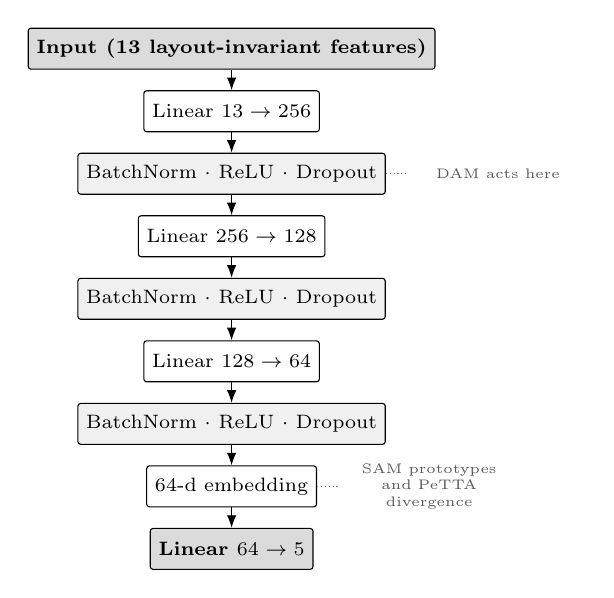
\begin{tikzpicture}[node distance=2.6mm]
  \node[io]                        (in)  {Input (13 layout-invariant features)};
  \node[blk, below=of in]          (l1)  {Linear $13 \rightarrow 256$};
  \node[shaded, below=of l1]       (b1)  {BatchNorm $\cdot$ ReLU $\cdot$ Dropout};
  \node[blk, below=of b1]          (l2)  {Linear $256 \rightarrow 128$};
  \node[shaded, below=of l2]       (b2)  {BatchNorm $\cdot$ ReLU $\cdot$ Dropout};
  \node[blk, below=of b2]          (l3)  {Linear $128 \rightarrow 64$};
  \node[shaded, below=of l3]       (b3)  {BatchNorm $\cdot$ ReLU $\cdot$ Dropout};
  \node[blk, below=of b3]          (emb) {64-d embedding};
  \node[io, below=of emb]          (out) {Linear $64 \rightarrow 5$};
  \foreach \a/\b in {in/l1, l1/b1, b1/l2, l2/b2, b2/l3, l3/b3, b3/emb, emb/out}
    \draw[ar] (\a) -- (\b);
  \node[note, right=3mm of b1, text width=20mm] {DAM acts here};
  \node[note, right=3mm of emb, text width=20mm] {SAM prototypes\\ and PeTTA\\ divergence};
  \draw[densely dotted, black!50] (b1.east) -- ++(2.6mm,0);
  \draw[densely dotted, black!50] (emb.east) -- ++(2.6mm,0);
\end{tikzpicture}}

% ---------------------------------------------------------------- Fig: DIGA
\newcommand{\figDIGA}{%
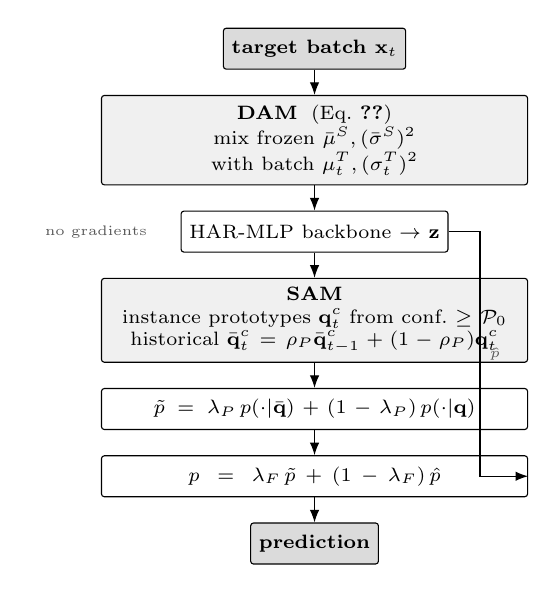
\begin{tikzpicture}[node distance=3.2mm]
  \node[io]                               (x)   {target batch $\mathbf{x}_t$};
  \node[shaded, below=of x, text width=52mm] (dam)
       {\textbf{DAM} \;(Eq.~\ref{eq:dam})\\
        mix frozen $\bar\mu^S,(\bar\sigma^S)^2$ with batch $\mu^T_t,(\sigma^T_t)^2$};
  \node[blk, below=of dam]                (bb)  {HAR-MLP backbone $\rightarrow$ $\mathbf{z}$};
  \node[shaded, below=of bb, text width=52mm] (sam)
       {\textbf{SAM}\\
        instance prototypes $\mathbf{q}^c_t$ from conf.\ $\geq\mathcal{P}_0$\\
        historical $\bar{\mathbf{q}}^c_t=\rho_P\bar{\mathbf{q}}^c_{t-1}+(1-\rho_P)\mathbf{q}^c_t$};
  \node[blk, below=of sam, text width=52mm] (mix)
       {$\tilde p=\lambda_P\,p(\cdot|\bar{\mathbf{q}})+(1-\lambda_P)\,p(\cdot|\mathbf{q})$};
  \node[blk, below=of mix, text width=52mm] (fus)
       {$p=\lambda_F\,\tilde p+(1-\lambda_F)\,\hat p$};
  \node[io, below=of fus]                 (y)   {prediction};
  \foreach \a/\b in {x/dam, dam/bb, bb/sam, sam/mix, mix/fus, fus/y}
    \draw[ar] (\a) -- (\b);
  \draw[ar] (bb.east) -- ++(4mm,0) |- (fus.east) node[note, pos=0.25, right=0pt]
       {$\hat p$};
  \node[note, left=2mm of bb, text width=15mm] {no gradients};
\end{tikzpicture}}

% ---------------------------------------------------------------- Fig: PETAL
\newcommand{\figPETAL}{%
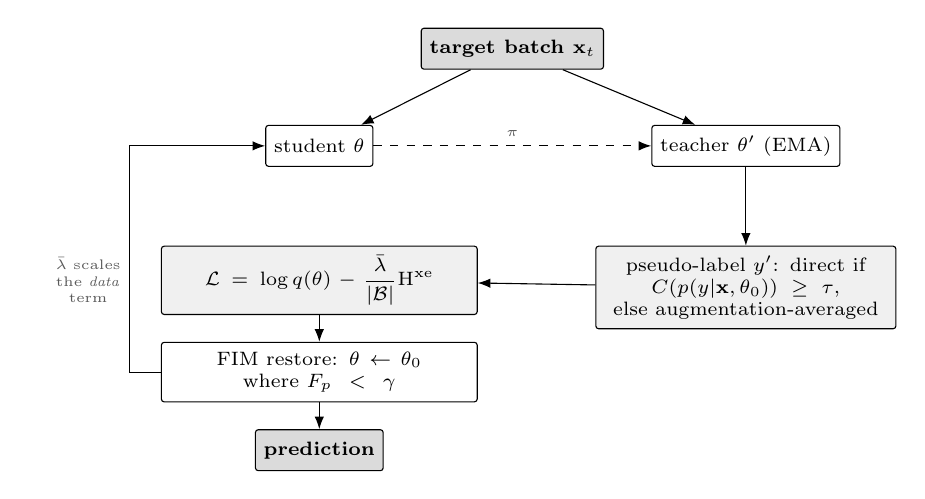
\begin{tikzpicture}[node distance=3.4mm]
  \node[io]                                (x)  {target batch $\mathbf{x}_t$};
  \node[blk, below left=7mm and 6mm of x]  (st) {student $\theta$};
  \node[blk, below right=7mm and 6mm of x] (te) {teacher $\theta'$ (EMA)};
  \draw[ar] (x) -- (st); \draw[ar] (x) -- (te);
  \draw[arb] (st) -- node[note, above] {$\pi$} (te);

  \node[shaded, below=10mm of te, text width=36mm] (pl)
       {pseudo-label $y'$: direct if\\ $C(p(y|\mathbf{x},\theta_0))\geq\tau$,\\
        else augmentation-averaged};
  \draw[ar] (te) -- (pl);

  \node[shaded, below=10mm of st, text width=38mm] (ls)
       {$\mathcal{L}=\log q(\theta)-\dfrac{\bar\lambda}{|\mathcal{B}|}\mathrm{H}^{\mathrm{xe}}$};
  \draw[ar] (pl) -- (ls);
  \node[note, left=1.5mm of ls, text width=13mm] {$\bar\lambda$ scales\\ the \emph{data}\\ term};

  \node[blk, below=of ls, text width=38mm] (fim)
       {FIM restore: $\theta\!\leftarrow\!\theta_0$ where $F_p<\gamma$};
  \draw[ar] (ls) -- (fim);
  \draw[ar] (fim.west) -- ++(-4mm,0) |- (st.west);
  \node[io, below=of fim] (y) {prediction};
  \draw[ar] (fim) -- (y);
\end{tikzpicture}}

% ---------------------------------------------------------------- Fig: PeTTA
\newcommand{\figPeTTA}{%
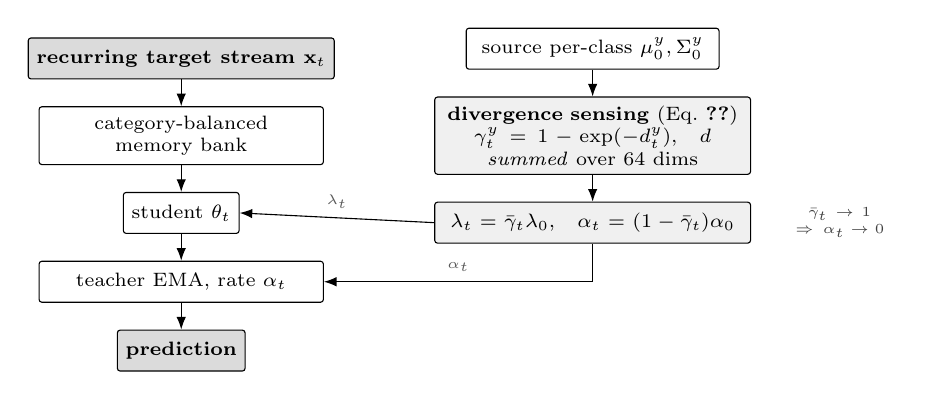
\begin{tikzpicture}[node distance=3.4mm]
  \node[io]                                 (x)  {recurring target stream $\mathbf{x}_t$};
  \node[blk, below=of x, text width=34mm]   (bank) {category-balanced memory bank};
  \node[blk, below=of bank]                 (st)  {student $\theta_t$};
  \node[shaded, right=14mm of bank, text width=38mm] (div)
       {\textbf{divergence sensing} (Eq.~\ref{eq:petta-gamma})\\
        $\gamma^y_t=1-\exp(-d^y_t)$,\quad $d$ \emph{summed} over 64 dims};
  \node[shaded, below=of div, text width=38mm] (ada)
       {$\lambda_t=\bar\gamma_t\lambda_0$,\quad $\alpha_t=(1-\bar\gamma_t)\alpha_0$};
  \node[blk, above=of div, text width=30mm] (src)
       {source per-class $\mu^y_0,\Sigma^y_0$};
  \node[blk, below=of st, text width=34mm]  (te)
       {teacher EMA, rate $\alpha_t$};
  \node[io, below=of te]                    (y)   {prediction};
  \foreach \a/\b in {x/bank, bank/st, st/te, te/y} \draw[ar] (\a) -- (\b);
  \draw[ar] (src) -- (div);
  \draw[ar] (div) -- (ada);
  \draw[ar] (ada.west) -- node[note, above, pos=0.5] {$\lambda_t$} (st.east);
  \draw[ar] (ada.south) |- node[note, above, pos=0.75] {$\alpha_t$} (te.east);
  \node[note, right=1.5mm of ada, text width=17mm, text=black!75]
       {$\bar\gamma_t\!\to\!1$\\ $\Rightarrow \alpha_t\!\to\!0$};
\end{tikzpicture}}


\begin{document}

\let\WriteBookmarks\relax
\def\floatpagepagefraction{1}
\def\textpagefraction{.001}

\shorttitle{Sensor identity does not transfer}
\shortauthors{M. Kbaier et al.}

\title[mode=title]{Sensor Identity Does Not Transfer: Revisiting Test-Time
Adaptation for Cross-Building Human Activity Recognition}

\author[1]{Mariem Kbaier}
\ead{kbaiermeryem@gmail.com}

\author[1]{Ons Abderrahim}

\author[1]{Manar Amayri}

\author[1]{Nizar Bouguila}
\cormark[1]
\ead{nizar.bouguila@concordia.ca}

\affiliation[1]{organization={Concordia Institute for Information Systems
  Engineering, Concordia University},
  city={Montreal}, state={QC}, country={Canada}}

\cortext[1]{Corresponding author.}

\begin{abstract}
Test-time adaptation (TTA) is an appealing answer to cross-building deployment in smart
buildings: sensors run continuously, and labelled data from a new site never arrives. We
set out to evaluate three TTA methods developed for images --- DIGA, PETAL and PeTTA ---
on human activity recognition and occupancy estimation across buildings, and found first
that the evaluation protocol itself was the dominant effect. Sliding windows with unit
stride cause adjacent samples to share nineteen of twenty timesteps, so a random
train/validation split places a near-duplicate of almost every validation sample into
training. Under that split a source model reaches $0.998$ \macf; grouped by recording day
it reaches $0.53$. The window definition makes almost no difference to this: the inflation
comes from the split.

Measured consistently, the cross-building drop is far smaller than reported. With causal
windows that an online system can compute, and features that do not encode sensor
identity, source and target \macf{} are $0.534$ and $0.447$ in one transfer direction and
$0.454$ and $0.307$ in the reverse --- a gap of $9$ to $15$ points rather than $83$. The
features responsible are thirteen window-level summary statistics. The $106$ per-sensor
features that dominate the usual design score \emph{below} stratified-random guessing on
the target in both directions, because a given sensor index is a different physical device
in each building. One pattern recurs across every design choice we varied --- which features, how long
the window, how much temporal context --- and in both transfer directions: the
configuration that validates best in-domain transfers worst. On this data, selecting a
model by in-domain accuracy selects the worst one to deploy elsewhere; whether that holds
beyond these two apartments is untested.

Against that baseline the three methods behave differently, and each failure
traces to a specific published equation rather than to our port. PETAL's coefficient
weights the likelihood, so the value selected by tuning on target labels removes the
learning signal entirely. PeTTA gates its update rate on a Mahalanobis distance summed
over $64$ embedding dimensions; across buildings that sum is large enough that the gate
saturates and the teacher stops updating. DIGA does help, by $1.7$ \macf{} points with a
bootstrap interval excluding zero, but only with hyperparameters retuned on target labels.
Occupancy estimation then supplies the clearest test, because the two transfer
directions differ only in the quality of the source checkpoint. Against a sound one no
method improves and the normalisation-based ones lose ground; against a checkpoint that is
worse than chance the same methods gain $27$ to $41$ MCC points. Adaptation gain here
measures source-model deficiency, not adaptation quality. Our conclusion is not that TTA fails in smart
buildings, but that it was being asked to repair a problem largely created by evaluation
and feature design.
\end{abstract}

\begin{keywords}
Test-time adaptation \sep Human activity recognition \sep Occupancy estimation \sep
Smart buildings \sep Evaluation leakage \sep Domain adaptation
\end{keywords}

\maketitle

% ============================================================================
\section{Introduction}
\label{sec:intro}

Buildings account for a large share of global energy demand, and occupancy-aware control
of HVAC and lighting is one of the more direct levers available for reducing it
\cite{manfren2021,amangeldy2025}. Human activity recognition (HAR) and occupancy
estimation (OE) supply the signal such control needs \cite{dridi2022,amayri2019}. Both are
learned from sensor traces, and both face the same obstacle when a model trained in one
building is installed in another: room layouts differ, sensors sit in different places,
and occupants keep different routines \cite{shahbazian2023,hong2017}. A model that works
in the building where it was trained often does not work in the next one.

Test-time adaptation addresses this without requiring labels from the new site. A frozen
source model updates itself online from the unlabelled stream it is already processing,
with no access to source data and no target annotation \cite{liang2024}. For buildings,
where sensors are always on and manual annotation is impractical, the fit is obvious. The
method family has matured quickly on images: DIGA \cite{diga} adapts normalisation
statistics and class prototypes without gradients, PETAL \cite{petal} treats lifelong
adaptation as probabilistic inference, and PeTTA \cite{petta} stabilises adaptation when
environments recur. Whether their assumptions survive the move to one-dimensional sensor
data is an open question, and the one we set out to answer.

We did not answer it in the form we expected. Our first experiments reproduced the
standard pipeline and produced the standard picture: a source model validating near
$0.99$ \macf{} and collapsing to $0.16$ on a second apartment, which reads as severe
domain shift. Most of that drop turned out to be an artefact of how the validation split
was constructed. Features are computed over sliding windows with unit stride, so
consecutive samples share $19$ of their $20$ timesteps; a random split puts a
$95\%$-identical copy of nearly every validation sample into training. Grouping the split
by recording day instead --- a one-line change --- moves source validation from $0.998$ to
$0.53$ and leaves the target number essentially untouched. The gap that motivates this
literature shrinks accordingly.

Once the protocol is fixed, the picture changes in a way that is more interesting than
the original. Most of the remaining gap is attributable not to some irreducible property
of cross-building transfer but to the features themselves. The conventional design devotes
$106$ of its $135$ dimensions to per-sensor statistics, and those features are actively
harmful across buildings: used alone they score below chance in both transfer directions,
because \texttt{sensor\_id\_100} is a different physical device in each apartment. A model
built from thirteen layout-invariant window statistics transfers far better while
validating slightly worse in-domain.

That inversion is the central finding of this paper, and it is not confined to the choice
of features. We observed it four more times, in both transfer directions: longer windows
validate better and transfer worse; added temporal context does the same; and in the
reverse direction the conventional feature vector attains the best source-validation
score of any configuration we tried and the worst target score, below chance. The
practical consequence is immediate and uncomfortable. Choosing a checkpoint by in-domain
validation --- the ordinary thing to do --- systematically picks the model that will
perform worst in the next building.

What remains for adaptation to do is correspondingly small, and the three methods divide
cleanly. One helps a little. Two do not run at all, and in both cases the reason is
specific, mechanical, and traceable to an equation in the original paper rather than to
our implementation.

Our contributions are as follows.

\begin{itemize}
\item \textbf{A protocol error that accounts for most of the reported cross-building gap.}
  We isolate it by varying the window definition and the validation split independently.
  Causality and segmentation move source \macf{} by less than two points; the split moves
  it by forty-six (Section~\ref{sec:res-leak}).

\item \textbf{Causal features that are both deployable and better.} Windows centred on the
  labelled sample read five minutes into the future, contradicting the online premise of
  TTA. Replacing them with causal windows improves target \macf{} by $7.3$ points. There
  is no trade-off to manage (Section~\ref{sec:res-leak}).

\item \textbf{In-domain fit anti-correlates with cross-building transfer}, shown across
  feature sets, window length and temporal context, in both transfer directions
  (Sections~\ref{sec:res-feat} and~\ref{sec:res-ceiling}). Per-sensor features, which
  drive most of the effect, score below stratified-random on the target either way.

\item \textbf{A located ceiling.} Seven attempts to raise target performance beyond the
  deployable checkpoint are reported, six of which fail, including an unsupervised
  sensor-correspondence method given the advantage of offline access to the target
  stream (Sections~\ref{sec:res-ceiling} and~\ref{sec:res-corr}).

\item \textbf{Three mechanisms by which image-domain assumptions break on sensor data},
  each tied to a published equation: PETAL's $\bar\lambda$ scales the likelihood, PeTTA's
  divergence signal saturates, and DIGA's advertised global hyperparameters do not
  transfer (Section~\ref{sec:res-mech}).

\item \textbf{A second task isolating what adaptation gain measures.} On cross-office
  occupancy estimation the two transfer directions differ only in the quality of the
  source checkpoint: against a sound one no method improves, against one worse than
  chance the same methods gain $27$ to $41$ MCC points. PETAL and PeTTA reproduce source
  predictions in both (Section~\ref{sec:res-oe}).
\end{itemize}

Section~\ref{sec:related} reviews domain adaptation and TTA for sensor data.
Section~\ref{sec:background} states the problem and the three methods.
Section~\ref{sec:method} describes our data handling, protocol and features.
Sections~\ref{sec:setup} and~\ref{sec:results} give the setup and results.
Sections~\ref{sec:discussion} and~\ref{sec:conclusion} discuss and conclude.

% ============================================================================
\section{Related work}
\label{sec:related}

\subsection{Domain adaptation in smart buildings}

Cross-environment degradation in building sensor models is well documented, and the usual
remedy is feature-level alignment using unlabelled target data gathered before deployment
\cite{dridi2022,abderrahim2025,amayri2019}. Open-set extensions handle activities present
in the target but absent from source training \cite{abderrahim2026,abderrahim_osda}. What
these approaches share is an offline phase: target data must be collected and processed
before the model goes live. A model arriving in a new building has none, annotating sensor
streams is expensive, and taking a building management system offline to retrain is rarely
acceptable. TTA exists to remove that phase.

\subsection{Test-time adaptation and its assumptions}

TTA adapts a pre-trained model during inference using only unlabelled target samples
\cite{liang2024}. It is stricter than source-free domain adaptation \cite{shot}, which
permits repeated offline passes over the target set: TTA runs online, in a single pass, on
samples as they arrive. TENT \cite{tent} minimises prediction entropy over batch
normalisation parameters and assumes a stationary, i.i.d.\ test stream --- both of which
fail for building sensors, where distributions drift across the day and consecutive
readings are correlated. Under class imbalance, entropy minimisation tends to reinforce
the majority class, since confident low-entropy outputs are easiest to produce for
frequent classes. CoTTA \cite{cotta} extends TENT to continual settings with weight
averaging and stochastic restoration, but relies on augmentation-averaged pseudo-labels,
for which one-dimensional sensor data has no natural analogue.

The three methods we study were selected because their mechanisms are, at least in
principle, modality-agnostic. DIGA \cite{diga} mixes source and instance normalisation
statistics and adds a prototype classifier, computing no gradients at all. PETAL
\cite{petal} places a posterior over source weights and derives a student--teacher
objective with a source-posterior regulariser and Fisher-information-based restoration.
PeTTA \cite{petta} targets recurring environments (Fig.~\ref{fig:petta}), monitoring drift from the source model
and modulating its adaptation rate to prevent collapse. Section~\ref{sec:res-mech} shows
that each nonetheless embeds an assumption that fails here.

\subsection{TTA for one-dimensional data}

Outside vision, TTA is comparatively unexplored. Wang et al.~\cite{wang2023} propose an
optimisation-free method for wearable HAR using exponential-decay test-time
normalisation. Related work studies source-free adaptation for EEG, which shares temporal
correlation and channel heterogeneity with building sensors. None of this work addresses
the combination we face: severe class imbalance, differing sensor layouts across sites,
and recurring daily structure. Nor, to our knowledge, has any prior study examined how
evaluation protocol and feature design interact with measured adaptation gains ---
which, as we show, dominates the comparison.

% ============================================================================
\section{Background}
\label{sec:background}

\subsection{Problem formulation}

A domain is a pair $\mathcal{D}=(\mathcal{X},P(X))$ with feature space $\mathcal{X}$ and
input marginal $P(X)$. A model $f_\theta$ is trained on a source domain
$\mathcal{D}_S=(\mathcal{X}_S,P_S(X))$ from labelled data $\{(\mathbf{x}_n,y_n)\}_{n=1}^N$
and deployed on a target $\mathcal{D}_T$ with $P_S(X)\neq P_T(X)$ and no labels. At step
$t$ the model receives $\mathbf{x}_t\in\mathcal{X}_T$, predicts
$\hat y_t=f_{\theta_t}(\mathbf{x}_t)$, and updates $\theta_{t-1}\to\theta_t$ without
seeing a label:
\begin{equation}
\min_{\theta}\;
\mathbb{E}_{\mathbf{x}_t\sim P_T(X)}\big[\mathcal{L}_{\mathrm{TTA}}(f_\theta(\mathbf{x}_t))\big]
+\mathcal{R}(\theta,\theta_0),
\label{eq:tta}
\end{equation}
where $\theta_0$ are the source parameters and $\mathcal{R}$ penalises drift.

Two constraints on Eq.~\ref{eq:tta} are usually left implicit and matter a great deal
here. First, $f_{\theta_t}(\mathbf{x}_t)$ must be computable from information available at
time $t$; a feature that reads future samples cannot be deployed. Second, any quantity
used to define $\mathcal{X}$ --- scalers, pruning masks, prototypes --- must be estimable
without target labels, and ideally without target data. Section~\ref{sec:method} enforces
both.

\subsection{DIGA}

DIGA \cite{diga}, summarised in Fig.~\ref{fig:diga}, combines a Distribution Adaptation Module (DAM) and a Semantic Adaptation
Module (SAM), with no gradient computation. DAM mixes frozen source batch-normalisation
statistics with those of the current batch:
\begin{align}
\bar\mu^{T}_t &= \lambda_{\mathrm{BN}}\bar\mu^{S}+(1-\lambda_{\mathrm{BN}})\mu^{T}_t, \nonumber\\
(\bar\sigma^{T}_t)^2 &= \lambda_{\mathrm{BN}}(\bar\sigma^{S})^2+(1-\lambda_{\mathrm{BN}})(\sigma^{T}_t)^2 .
\label{eq:dam}
\end{align}
SAM estimates per-class prototypes $\mathbf{q}^c_t$ from predictions above confidence
$\mathcal{P}_0$, carries a historical copy by exponential moving average,
$\bar{\mathbf{q}}^c_t=\rho_P\bar{\mathbf{q}}^c_{t-1}+(1-\rho_P)\mathbf{q}^c_t$, and builds
\emph{two} non-parametric classifiers which are mixed by $\lambda_P$ before being fused
with the parametric output by $\lambda_F$:
\begin{align}
\tilde p &= \lambda_P\,p(c|\mathbf{x}_t,\bar{\mathbf{q}})+(1-\lambda_P)\,p(c|\mathbf{x}_t,\mathbf{q}), \\
p &= \lambda_F\,\tilde p+(1-\lambda_F)\,\hat p .
\label{eq:diga-fuse}
\end{align}
We note that DIGA's Eq.~8 writes $p(c|\mathbf{x},\mathbf{q})\propto\exp(-\langle
\mathbf{z},\mathbf{q}_c\rangle)$. Read literally as an inner product this ranks the
\emph{least} similar prototype highest; we therefore treat $\langle\cdot,\cdot\rangle$ as
a dissimilarity and report the effect of the alternatives in
Section~\ref{sec:res-mech}.


\begin{figure}[t]
\centering
\resizebox{0.95\columnwidth}{!}{\figDIGA}
\caption{DIGA applied to the one-dimensional backbone. DAM mixes frozen source
batch-normalisation statistics with the current batch's; SAM builds instance and
historical prototypes and fuses their predictions with the parametric classifier. No
gradient is computed anywhere in the loop.}
\label{fig:diga}
\end{figure}

\subsection{PETAL}

PETAL \cite{petal}, shown in Fig.~\ref{fig:petal}, approximates the source posterior $q(\theta)$ by SWAG-diagonal and
updates a student by ascending
\begin{equation}
\mathcal{L}=\log q(\theta)-\frac{\bar\lambda}{|\mathcal{B}|}\,
\mathrm{H}^{\mathrm{xe}}(y',y\,|\,\bar{\mathbf{x}}),
\qquad \theta_{t+1}=\theta_t+\eta\nabla_\theta\mathcal{L},
\label{eq:petal}
\end{equation}
with pseudo-labels $y'$ from an EMA teacher and a Fisher-information criterion restoring
unimportant parameters to $\theta_0$. The role of $\bar\lambda$ in Eq.~\ref{eq:petal} is
worth stating explicitly, because it is easy to misread: $\bar\lambda$ multiplies the
\emph{data} term, and the prior weight is fixed at unity. Setting $\bar\lambda=0$ does not
remove a regulariser; it removes the likelihood, leaving an update that does not depend on
the target stream at all.


\begin{figure*}[t]
\centering
\resizebox{0.80\textwidth}{!}{\figPETAL}
\caption{PETAL's student--teacher loop. The coefficient $\bar\lambda$ multiplies the
cross-entropy, not the source-posterior term; Section~\ref{sec:res-mech} shows what
follows when it is set to zero.}
\label{fig:petal}
\end{figure*}

\subsection{PeTTA}

PeTTA \cite{petta} targets recurring environments. It senses divergence in feature space
through a Mahalanobis distance between per-class running means and their source
counterparts,
\begin{equation}
\gamma^y_t=1-\exp\!\big(-(\hat\mu^y_t-\mu^y_0)^\top(\Sigma^y_0)^{-1}(\hat\mu^y_t-\mu^y_0)\big),
\label{eq:petta-gamma}
\end{equation}
and uses the batch average $\bar\gamma_t$ to set both the regularisation weight and the
teacher update rate,
\begin{equation}
\lambda_t=\bar\gamma_t\lambda_0,\qquad \alpha_t=(1-\bar\gamma_t)\alpha_0 .
\label{eq:petta-alpha}
\end{equation}
The quadratic form in Eq.~\ref{eq:petta-gamma} is a \emph{sum} over embedding dimensions.
Section~\ref{sec:res-mech} shows what that implies when the two domains are different
buildings rather than corruptions of the same image.


\begin{figure*}[t]
\centering
\resizebox{0.86\textwidth}{!}{\figPeTTA}
\caption{PeTTA for recurring streams. A single scalar $\bar\gamma_t$, derived from a
Mahalanobis distance \emph{summed} over the embedding dimension, sets both the
regularisation weight and the teacher update rate. As $\bar\gamma_t\to1$ the update rate
goes to zero.}
\label{fig:petta}
\end{figure*}

% ============================================================================
\section{Methodology}
\label{sec:method}

\subsection{Windowing}
\label{sec:method-window}

Binary sensor activations are aggregated over windows of $W=20$ consecutive timesteps at
$30$\,s resolution, giving a $10$-minute window per labelled sample. Two choices in this
step are usually made implicitly, and we make both explicit because they turn out to
matter.

\paragraph{Causality.} A window may be \emph{centred} on the labelled sample, spanning
$[i-W/2,\,i+W/2]$, or \emph{causal}, spanning $[i-W+1,\,i]$. The centred form is common
and reads five minutes into the future of every sample, which is incompatible with online
deployment. We use causal windows throughout and quantify the difference in
Section~\ref{sec:res-leak}.

\paragraph{Segmentation.} Windows must be truncated somewhere. Segmenting on
\emph{ground-truth activity changes} guarantees that no window straddles two activities,
but hands the extractor the label transitions it is meant to predict. We segment instead
on \emph{recording continuity}: a new segment begins at a day change or a gap in the
$30$\,s sampling. This uses no labels and is what a deployed system can determine. Windows
are truncated at segment starts rather than dropped, which is what an online system
genuinely has after a gap.

\subsection{Validation protocol}
\label{sec:method-split}

Because stride is one, adjacent samples share $W-1$ of $W$ timesteps. A random
train/validation split therefore places a near-duplicate of nearly every validation sample
into training, and the resulting score measures memorisation rather than generalisation.
We use \textbf{GroupKFold over \texttt{year\_day}}: no recording day appears in both
halves, which removes window overlap and same-day correlation together. All source model
selection in this paper uses this protocol. Section~\ref{sec:res-leak} reports what each
alternative gives.

\subsection{Features}
\label{sec:method-feat}

The conventional $135$-dimensional vector comprises $106$ per-sensor statistics (mean and
standard deviation for each of the $53$ shared sensors), five window-level activity
statistics, $20$ co-activation indicators for the most frequent sensor pairs in the
source, and four cyclic time encodings. Of these, $126$ are tied to \emph{sensor
identity}: the index $100$ refers to a different physical device in each building, so a
rule learned about it is not merely uninformative in the target but wrong.

We therefore evaluate a $13$-dimensional \textbf{layout-invariant} set: nine window-level
statistics of the per-timestep active-sensor count (mean, maximum, minimum, median,
standard deviation, idle fraction, activation entropy, transition count, transition rate)
and four cyclic encodings of time of day and day of week. Nothing in this set refers to
which sensor fired. Appendix~A reports a larger invariant set including a sorted
activation profile and run-length structure; it does not improve on the thirteen.

Fig.~\ref{fig:pca} projects the engineered space onto its first two source principal
components; the target occupies a displaced, compressed region.

All transforms are fitted on the source training split only. No target labels and no
target statistics are used at any point in constructing the source model, so every
configuration remains a legal TTA starting point.


\begin{figure}[t]
\centering
\resizebox{0.82\columnwidth}{!}{\figMLP}
\caption{The classifier used throughout. Only the input width changes between feature
sets; depth, widths and regularisation are held fixed so that comparisons isolate the
features.}
\label{fig:mlp}
\end{figure}

\begin{figure*}[t]
\centering
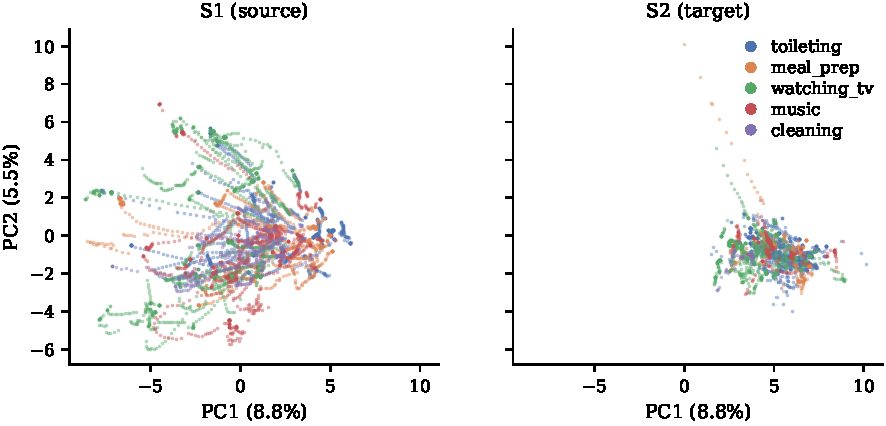
\includegraphics[width=0.92\textwidth]{fig_pca.pdf}
\caption{First two principal components of the causal engineered feature space, fitted on
S1 and applied unchanged to S2. The target occupies a displaced and markedly compressed
region, which is the shift the adaptation methods are asked to absorb.}
\label{fig:pca}
\end{figure*}

\subsection{Causal prediction smoothing}

Activities persist for minutes while predictions are made per $30$\,s window. We apply a
median filter over the last $L$ predictions, never crossing a recording-segment boundary.
This uses only past outputs and so remains deployable online. We report $L=41$, selected
on source data.

\subsection{Stream protocol}

Target data is divided into eight contiguous segments. \emph{Non-recurring} streams visit
each once; \emph{recurring} streams make three passes in randomised order, repeated over
three independent orderings. Target labels are withheld throughout adaptation and used
only to score predictions afterwards.

\subsection{What a method is allowed to know}
\label{sec:method-tiers}

Methods in this literature differ in what they require of the target building before they
can produce a prediction, and the distinction is usually left implicit. We separate three
levels.

\begin{description}
\item[Tier 1, no target data.] Everything is estimated on the source. The model can be
  installed in a new building and run immediately. This is the setting test-time
  adaptation exists to serve.
\item[Tier 2, unlabelled target data, offline.] The full target distribution must be
  collected before deployment, though no labels are needed. This is source-free domain
  adaptation. It is a weaker requirement than labels but it reintroduces exactly the
  data-collection phase that motivates TTA.
\item[Tier 3, target labels.] Not deployable.
\end{description}

The distinction matters for what follows. The layout-invariant features used throughout
this paper are tier 1: every transform is fitted on the source split alone, and the model
needs nothing from the target building. Feature-shift pruning, by contrast, selects
features by comparing source and target distributions, and is therefore tier 2 ---
unsupervised, but not deployable without a prior observation period. The hyperparameter
selection discussed next is tier 3.

\subsection{Hyperparameter selection}
\label{sec:method-hparam}

We report results using each method's \emph{published} hyperparameters, and separately
under target-label tuning where the two differ materially. Selecting on target labels is
not available in deployment, and Section~\ref{sec:res-mech} shows it can actively select a
degenerate configuration. Where a label-free criterion is needed we use mean prediction
entropy on the target stream.

% ============================================================================
\section{Experimental setup}
\label{sec:setup}

\subsection{Datasets}

\paragraph{HAR.} The dataset of \citet{tapia2004} provides two single-occupant
apartments, S1 and S2, instrumented with binary proximity sensors on household objects and
recorded over roughly two weeks each ($16$ recording days here). S1 exposes $70$ sensor columns and S2 exposes $75$; feature engineering uses the
$53$ shared by both. Table~\ref{tab:har-data} gives per-class counts. We evaluate both
transfer directions.

Class names follow the source annotation (\texttt{toileting}, \texttt{meal\_prep},
\texttt{watching\_tv}, \texttt{music}, \texttt{cleaning}). We note this because the
time-of-day distributions confirm them: activity code $65$ occurs between 07:31 and 14:51
with a median of 11:34, which is consistent with \texttt{watching\_tv} and not with a
sleep-type label.

\paragraph{Occupancy.} A private dataset collected from two university offices (H355 and
H358) at the Grenoble Institute of Technology using CO\textsubscript{2} concentration
sensors \cite{dridi_cluster,amayri2019}. The original annotation records occupancy counts
(zero, one, two, three, more than three); we binarise to occupied / not occupied. The
representation is nine engineered features produced by the originating pipeline; we use
them as supplied and perform no further feature construction, so no target information
enters through any step we control. Splits are $1145$ / $200$ source train / test and
$822$ / $150$ target train / test, with roughly $78\%$ / $22\%$ class balance. Because
the data is private, the released code reproduces the HAR results only.

\begin{table*}[t]
\centering
\caption{HAR dataset statistics. Class names follow the source annotation.}
\label{tab:har-data}
\small
\begin{tabular}{lrrrrrr}
\toprule
Split & Total & toileting & meal\_prep & watching\_tv & music & cleaning \\
\midrule
S1 & 5031 & 1065 & 857 & 1598 & 1069 & 442 \\
S2 & 3412 & 1266 & 417 & 1291 & 325 & 113 \\
\bottomrule
\end{tabular}
\end{table*}

\subsection{Model}

A three-layer MLP with batch normalisation, ReLU and dropout (Fig.~\ref{fig:mlp}),
reducing the input to a $64$-dimensional embedding followed by a five-class output layer. The architecture is held
fixed across all feature sets so that comparisons isolate the features.

\subsection{Metrics and baselines}

We report accuracy, \macf, MCC \cite{chicco2020} and per-class F\textsubscript{1}. \macf{} is the primary
metric for HAR because it weights all activities equally, which matters when the target
minority classes are small.

Chance baselines are reported in every table and are not optional here: several published
figures for this transfer setting sit at or below them. On S2, constant-majority
prediction gives accuracy $0.378$ and \macf{} $0.110$, and stratified-random prediction
gives accuracy $0.306$ and \macf{} $\mathbf{0.200}$. On S1 the stratified-random \macf{} is
$0.200$. For binary occupancy, always predicting ``not occupied'' gives accuracy $0.773$,
\macf{} $0.436$ and MCC $0.000$.

Differences between methods are reported with $95\%$ paired bootstrap confidence
intervals over the target stream ($2000$ resamples), computed on the difference from
source-only.

% ============================================================================
\section{Results}
\label{sec:results}

\subsection{Decomposing the source-domain fit}
\label{sec:res-leak}

Table~\ref{tab:leak} and Fig.~\ref{fig:leakage} vary the window definition and the
validation split independently, holding the feature arithmetic fixed.

% source: results/exp4_windowing.csv  (src/exp4_windowing.py), 5 seeds
\begin{table*}[t]
\centering
\caption{Source-domain validation \macf{} by windowing policy and validation protocol
($135$ features, z-score, mean $\pm$ s.d.\ over 5 seeds). Reading down any column shows
that the window definition is nearly irrelevant; reading across any row shows that the
split is not.}
\label{tab:leak}
\small
\begin{tabular}{llccc}
\toprule
Causality & Segmentation & Random 80/20 & Blocked & Grouped by day \\
\midrule
centred & activity labels & $0.9984\pm0.0009$ & $0.4357\pm0.0345$ & $0.5287\pm0.0067$ \\
centred & recording       & $0.9979\pm0.0006$ & $0.4571\pm0.0451$ & $0.5258\pm0.0112$ \\
causal  & activity labels & $0.9975\pm0.0021$ & $0.4414\pm0.0131$ & $0.5261\pm0.0084$ \\
causal  & recording       & $0.9968\pm0.0022$ & $0.4608\pm0.0209$ & $0.5110\pm0.0115$ \\
\bottomrule
\end{tabular}
\end{table*}


\begin{figure*}[t]
\centering
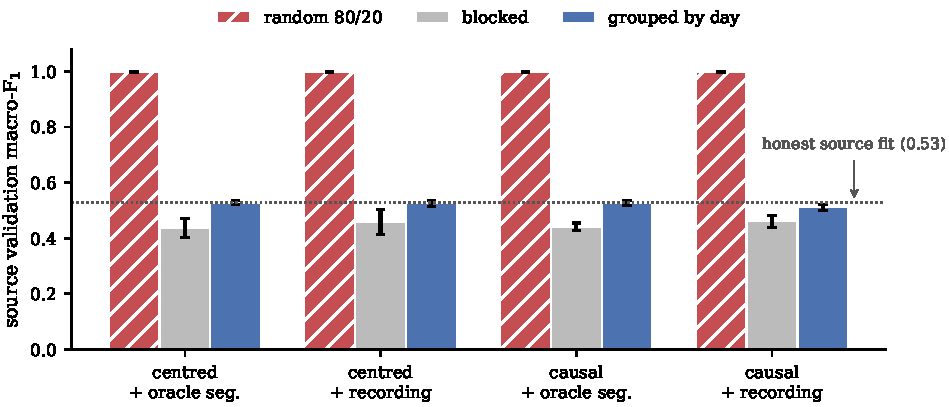
\includegraphics[width=0.92\textwidth]{fig_leakage.pdf}
\caption{Source validation \macf{} under every combination of windowing policy and
validation split (mean $\pm$ s.d.\ over 5 seeds). The hatched bars are the random split.
Its height is independent of how the window is defined, which locates the inflation in the
split rather than in the features.}
\label{fig:leakage}
\end{figure*}

A fully causal pipeline with no label-derived segmentation still validates at $0.9968$
under a random split. The inflation is therefore attributable to window overlap under
random splitting, not to the window definition. Grouping by recording day gives
$0.51$--$0.53$, and we treat that as the honest source-domain figure.

Causality nonetheless matters, in the opposite direction to what one might expect. Under
a fixed training protocol, making features causal \emph{improves} target transfer
(Table~\ref{tab:window-target}): \macf{} rises from $0.1626$ to $0.2356$, with accuracy
rising from $0.375$ to $0.444$. The deployable pipeline is also the better-transferring
one, so nothing is traded away by adopting it.

% source: results/exp4_windowing.csv
\begin{table*}[t]
\centering
\caption{Target transfer (S1$\to$S2) by windowing policy, $135$ features, blocked-trained,
mean over 5 seeds. Stratified-random \macf{} is $0.200$.}
\label{tab:window-target}
\small
\begin{tabular}{llccc}
\toprule
Causality & Segmentation & \macf & MCC & Accuracy \\
\midrule
centred & activity labels & $0.1626\pm0.0125$ & $0.0945$ & $0.3753$ \\
centred & recording       & $0.1953\pm0.0274$ & $0.1327$ & $0.3924$ \\
causal  & activity labels & $0.2344\pm0.0232$ & $0.2036$ & $0.4533$ \\
causal  & recording       & $\mathbf{0.2356}\pm0.0124$ & $0.1805$ & $0.4440$ \\
\bottomrule
\end{tabular}
\end{table*}

\subsection{Feature design}
\label{sec:res-feat}

Table~\ref{tab:features} sweeps feature subsets and source-fitted transforms on causal,
recording-segmented features under GroupKFold selection.

% source: results/exp5_features_causal_recording.csv (src/exp5_features_causal.py)
\begin{table*}[t]
\centering
\caption{S1$\to$S2 transfer by feature subset and source-fitted transform (causal
features, GroupKFold over 16 days, 5 seeds). Stratified-random \macf{} is $0.200$.}
\label{tab:features}
\small
\begin{tabular}{llcccc}
\toprule
Feature set & Transform & $d$ & Source-val \macf & Target \macf & Target MCC \\
\midrule
All (conventional)    & z-score     & 135 & $0.5083$ & $0.2436$ & $0.1682$ \\
All                   & rank-gauss  & 135 & $0.5890$ & $0.3775$ & $0.3144$ \\
KS-pruned 20\%        & z-score     & 108 & $0.5164$ & $0.3130$ & $0.2090$ \\
KS-pruned 20\%        & rank-gauss  & 108 & $\mathbf{0.6232}$ & $0.3004$ & $0.2138$ \\
No per-sensor         & z-score     & 29  & $0.5121$ & $0.3561$ & $0.2633$ \\
Global + temporal     & z-score     & 9   & $0.5341$ & $\mathbf{0.4133}$ & $\mathbf{0.3490}$ \\
Global only           & z-score     & 5   & $0.2914$ & $0.2129$ & $0.0970$ \\
Per-sensor only       & z-score     & 106 & $0.3292$ & $0.1484$ & $0.0436$ \\
\bottomrule
\end{tabular}
\end{table*}

Two observations. Per-sensor features alone reach $0.1484$ \macf, which is $5.1$ points
\emph{below} stratified-random guessing. They are not weakly informative; they encode
rules that are wrong in the target building. And the row with the best source-validation
score (KS-pruned with rank-gauss, $0.6232$) transfers at $0.3004$, while the row that
transfers best ($0.4133$) validates at $0.5341$. In-domain fit and cross-building transfer
pull in opposite directions, because what helps in-domain is precisely what is
building-specific.

Table~\ref{tab:both-dir} and Fig.~\ref{fig:features} repeat the comparison in both
directions.

% source: results/exp11_reverse.csv (src/exp11_reverse.py), 3 seeds x 5 folds
\begin{table*}[t]
\centering
\caption{Forward and reverse transfer under an identical protocol (causal features,
GroupKFold over the source's days, causal smoothing $L=41$). ``Gap'' is source-validation
minus target \macf, in points.}
\label{tab:both-dir}
\small
\begin{tabular}{llcccccc}
\toprule
Direction & Feature set & $d$ & Source-val & Target \macf & MCC & Gap & vs.\ chance \\
\midrule
S1$\to$S2 & Layout-invariant & 13  & $0.5341$ & $\mathbf{0.4466}$ & $0.3973$ & $8.8$  & $+24.7$ \\
S1$\to$S2 & All (conventional) & 135 & $0.5133$ & $0.2118$ & $0.0976$ & $30.2$ & $+1.2$ \\
S1$\to$S2 & Per-sensor only  & 106 & $0.3248$ & $0.1350$ & $0.0123$ & $19.0$ & $\mathbf{-6.5}$ \\
S1$\to$S2 & No per-sensor    & 29  & $0.5119$ & $0.3630$ & $0.2734$ & $14.9$ & $+16.3$ \\
\midrule
S2$\to$S1 & Layout-invariant & 13  & $0.4538$ & $\mathbf{0.3068}$ & $0.2667$ & $14.7$ & $+10.7$ \\
S2$\to$S1 & All (conventional) & 135 & $\mathbf{0.5381}$ & $0.1583$ & $0.0332$ & $38.0$ & $\mathbf{-4.2}$ \\
S2$\to$S1 & Per-sensor only  & 106 & $0.3668$ & $0.1702$ & $0.0553$ & $19.7$ & $\mathbf{-3.0}$ \\
S2$\to$S1 & No per-sensor    & 29  & $0.4483$ & $0.2271$ & $0.1043$ & $22.1$ & $+2.7$ \\
\bottomrule
\end{tabular}
\end{table*}


\begin{figure*}[t]
\centering
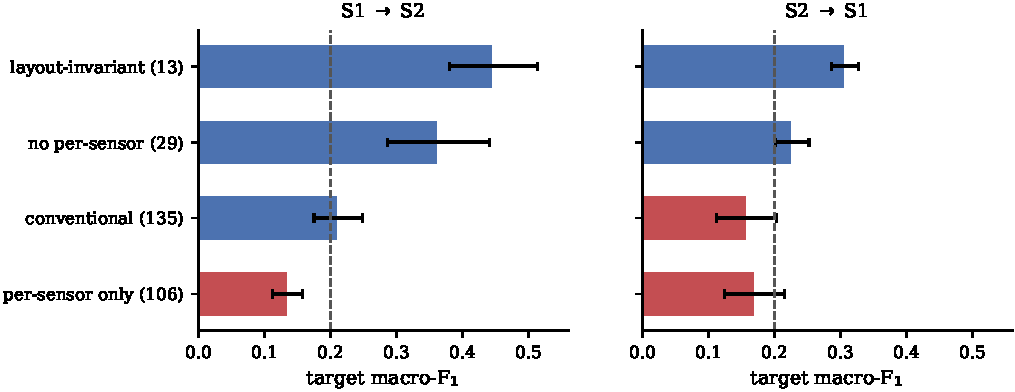
\includegraphics[width=0.92\textwidth]{fig_features.pdf}
\caption{Target \macf{} by feature set in both transfer directions, with the
stratified-random baseline marked (dashed). Bars falling short of it are shown in red.
Per-sensor features are below chance in both directions; the conventional 135-d vector is
below chance in one of them.}
\label{fig:features}
\end{figure*}

Both central claims replicate. Per-sensor features are below chance in both directions.
The inversion is sharper in reverse: the conventional $135$-d set has the best
source-validation score of any row ($0.5381$) and the worst transfer ($0.1583$), itself
$4.2$ points below chance.

The gap is direction-dependent: $8.8$ points forward and $14.7$ reverse. The asymmetry has
a visible cause rather than being noise. S2 is the weaker source --- $3412$ samples
against $5031$, with the hard classes much thinner ($113$ versus $442$ for
\texttt{cleaning}) --- and training on the smaller, more imbalanced apartment lowers both
sides of the comparison. We therefore state the result as a gap of $9$ to $15$ points
rather than quoting the more favourable direction.

\subsection{Test-time adaptation on the deployable checkpoint}
\label{sec:res-tta}

Table~\ref{tab:tta} compares the methods on the deployable checkpoint.

% source: results/exp6_tta_global+temporal.csv (src/exp6_tta_table.py), 3 seeds
\begin{table*}[t]
\centering
\caption{TTA on the layout-invariant causal checkpoint (3 seeds; recurring streams
additionally averaged over 3 randomised segment orderings). Stratified-random \macf{} is
$0.200$.}
\label{tab:tta}
\small
\begin{tabular}{llccc}
\toprule
Method & Stream & Accuracy & \macf & MCC \\
\midrule
Source-only & non-recurring & $0.6042\pm0.013$ & $0.4467\pm0.029$ & $0.4515\pm0.033$ \\
AdaBN       & non-recurring & $0.3782\pm0.011$ & $0.2977\pm0.005$ & $0.1517\pm0.013$ \\
TENT        & non-recurring & $0.3784\pm0.011$ & $0.2976\pm0.005$ & $0.1515\pm0.013$ \\
DIGA        & non-recurring & $0.6045\pm0.013$ & $\mathbf{0.4639}\pm0.001$ & $\mathbf{0.4739}\pm0.009$ \\
PETAL       & non-recurring & $0.6033\pm0.008$ & $0.4450\pm0.023$ & $0.4522\pm0.026$ \\
\midrule
Source-only & recurring & $0.6042\pm0.011$ & $0.4467\pm0.025$ & $0.4515\pm0.029$ \\
DIGA        & recurring & $\mathbf{0.6073}\pm0.010$ & $0.4625\pm0.013$ & $0.4700\pm0.022$ \\
PETAL       & recurring & $0.6038\pm0.010$ & $0.4431\pm0.020$ & $0.4504\pm0.026$ \\
PeTTA       & recurring & $0.6045\pm0.011$ & $0.4470\pm0.025$ & $0.4517\pm0.029$ \\
\bottomrule
\end{tabular}
\end{table*}

% source: results/exp6 bootstrap block
\begin{table*}[t]
\centering
\caption{$95\%$ paired bootstrap confidence intervals on the difference from source-only
($2000$ resamples, same stream).}
\label{tab:boot}
\small
\begin{tabular}{llcc}
\toprule
Method & Stream & $\Delta$\macf & $\Delta$MCC \\
\midrule
DIGA  & non-recurring & $[+0.0032,\,+0.0225]$ & $[+0.0277,\,+0.0559]$ \\
DIGA  & recurring     & $[+0.0146,\,+0.0311]$ & $[+0.0387,\,+0.0633]$ \\
PETAL & non-recurring & $[-0.0076,\,+0.0027]$ & $[-0.0013,\,+0.0130]$ \\
PETAL & recurring     & $[-0.0087,\,+0.0015]$ & $[-0.0067,\,+0.0067]$ \\
PeTTA & recurring     & $[-0.0007,\,+0.0006]$ & $[-0.0009,\,+0.0011]$ \\
AdaBN & non-recurring & $[-0.1754,\,-0.1379]$ & $[-0.3046,\,-0.2500]$ \\
TENT  & non-recurring & $[-0.1756,\,-0.1383]$ & $[-0.3050,\,-0.2503]$ \\
\bottomrule
\end{tabular}
\end{table*}

In Table~\ref{tab:boot}, DIGA is the only method whose interval excludes zero on the positive side, and the effect
is small: $+1.7$ \macf{} and $+2.2$ MCC points. For comparison, the feature redesign is
worth $+17.0$ \macf{} points before any adaptation runs. PETAL and PeTTA are statistically
indistinguishable from the unadapted model. AdaBN and TENT are substantially
\emph{worse} --- around $17$ points of \macf{} --- which is itself informative: adapting
normalisation statistics helps when the source model is poor and hurts once the features
are already distribution-robust.

Per-class F\textsubscript{1} (Table~\ref{tab:perclass}) shows four of five classes working.
DIGA's prototype correction does what it is designed to do, lifting \texttt{meal\_prep}
by eight points at a cost of seven on \texttt{toileting}. \texttt{cleaning}, with $113$
target samples, remains near zero for every method.

% source: results/exp6_tta_global+temporal.csv per-class columns
\begin{table*}[t]
\centering
\caption{Per-class F\textsubscript{1} on S2 (mean over seeds and orderings).}
\label{tab:perclass}
\small
\begin{tabular}{lccccc}
\toprule
Method & toileting & meal\_prep & watching\_tv & music & cleaning \\
\midrule
Source-only & $0.551$ & $0.493$ & $0.746$ & $0.435$ & $0.009$ \\
DIGA        & $0.478$ & $\mathbf{0.572}$ & $\mathbf{0.766}$ & $\mathbf{0.468}$ & $0.035$ \\
PETAL       & $0.550$ & $0.474$ & $0.746$ & $0.440$ & $0.014$ \\
PeTTA       & $0.552$ & $0.494$ & $0.746$ & $0.434$ & $0.009$ \\
AdaBN       & $0.365$ & $0.310$ & $0.482$ & $0.275$ & $0.056$ \\
\bottomrule
\end{tabular}
\end{table*}

\subsection{What does not move the result}
\label{sec:res-ceiling}

Target performance is bounded by source performance: the deployable checkpoint validates
at $0.534$ in-domain and transfers at $0.447$, a gap of under nine points. Raising the
target therefore requires raising the source with features that still cross buildings. We
report seven attempts, all negative, because together they locate the ceiling.

% source: results/exp10_improve.csv, exp15_classifier.csv, exp16_temporal.csv,
%         exp14_correspondence.csv
\begin{table*}[t]
\centering
\caption{Attempts to raise target \macf{} beyond the $13$-d causal checkpoint
(S1$\to$S2, same protocol throughout). Only causal smoothing and a source-estimated
transition model help, and both marginally.}
\label{tab:ceiling}
\small
\begin{tabular}{llcc}
\toprule
Attempt & What was varied & Source-val & Target \macf \\
\midrule
\textbf{baseline} & $13$-d, MLP, $W{=}20$, median $L{=}41$ & $0.5341$ & $\mathbf{0.4466}$ \\
\midrule
richer invariant features & $+$ sorted profile, runs, multi-scale ($60$-d) & $-$ & $0.4188$ \\
class weighting           & inverse-frequency weights          & $-$ & $0.3852$ \\
network width             & $64$--$32$ and $128$--$64$         & $-$ & $0.4297$ \\
classifier family         & boosting, forests, linear          & $0.5230$ & $0.4190$ \\
window length             & $W\in\{10,40,60\}$                 & $0.5611$ & $0.4330$ \\
temporal context          & stacked $T{=}11$, causal TCN $T{=}21$ & $0.5414$ & $0.4111$ \\
sensor correspondence     & unsupervised assignment (\S\ref{sec:res-corr}) & $-$ & $0.2227$ \\
\midrule
transition model          & source-estimated HMM, causal filtering & $0.5341$ & $0.4503$ \\
\bottomrule
\end{tabular}
\end{table*}

Two things are worth drawing out of Table~\ref{tab:ceiling}.

First, the only attempt that helps in \emph{both} transfer directions is the transition
model, and it helps by less than a point ($0.4466\to0.4503$ forward, $0.3068\to0.3160$
reverse). Its transition matrix is estimated on the source apartment and encodes nothing
about sensors --- only how often one activity follows another. That it transfers at all,
while every attempt to extract more from the sensor stream does not, is consistent with
the rest of this paper: what crosses buildings is behavioural regularity, not layout.

Second, and more importantly, several rows raise the source-validation score while
lowering the target. Window length does ($0.5611$ at $W{=}60$ against $0.5341$ at
$W{=}20$), and so does temporal context ($0.5414$ for the TCN). Section~\ref{sec:res-feat}
observed the same thing across feature sets. The pattern is general, and
Section~\ref{sec:discussion} returns to it.

\subsection{Can the sensors be matched across buildings?}
\label{sec:res-corr}

If per-sensor features fail only because index $100$ denotes a different device in each
apartment, the obvious repair is to estimate the correspondence. We tested this. Each
sensor was described by a behavioural signature computed from unlabelled data --- firing
rate, burst-length statistics, a $24$-bin diurnal profile, and an index-free summary of
its co-activation neighbourhood --- and the two sensor sets were matched by balanced
assignment on signature distance.

To separate a real correspondence from overfitting, permutations were estimated on one
half of the target stream and scored on the other.

% source: results/exp14_correspondence.csv and the half-split control
\begin{table}[t]
\centering
\caption{Per-sensor features under four permutations, target \macf. A correspondence that
is real should transfer between halves of the target stream.}
\label{tab:corr}
\small
\begin{tabular}{lcc}
\toprule
Permutation & Fitted half & Held-out half \\
\midrule
identity (no matching)      & $0.0976$ & $0.1744$ \\
learned signatures          & $0.0749$ & $0.2348$ \\
greedy search on fitted half& $\mathbf{0.4174}$ & $0.1738$ \\
random, 20 draws            & --- & $0.1655\pm0.050$ \\
\bottomrule
\end{tabular}
\end{table}

A greedy search reaches $0.417$ on the half it is fitted to and $0.174$ on held-out data,
indistinguishable from identity and from random. The signature-based assignment is
inconsistent between halves. No permutation we could find transfers.

We note that this test is permissive: estimating a correspondence from the whole
unlabelled target stream is offline source-free adaptation, not test-time adaptation
(Section~\ref{sec:method-tiers}), so it has an advantage no deployable method would have.
Failing under relaxed assumptions implies failing under strict ones.

The conclusion is stronger than the premise it tests. Per-sensor features do not fail
because they are mislabelled across buildings. They fail because a sensor in one
apartment has no counterpart in the other: rooms differ in shape, furniture sits
elsewhere, and routines differ. Relabelling cannot recover information that was never
shared.

\subsection{Three mechanisms}
\label{sec:res-mech}

\paragraph{PETAL: the coefficient scales the likelihood.} As noted in
Eq.~\ref{eq:petal}, $\bar\lambda$ weights the data term. Table~\ref{tab:lambda} sweeps it
on the deployable checkpoint with a non-degenerate SWAG posterior.

% source: results/exp12_lambda_bar.csv (src/exp12_lambda_bar.py)
\begin{table*}[t]
\centering
\caption{PETAL as a function of $\bar\lambda$ (published parameterisation,
Eq.~\ref{eq:petal}). Source-only is \macf{} $0.4641$, MCC $0.4679$. At $\bar\lambda=0$
the weights still move --- toward the SWAG mean --- but the movement is independent of
the target stream.}
\label{tab:lambda}
\small
\begin{tabular}{lcccc}
\toprule
$\bar\lambda$ & Drift from source & Predictions changed & \macf & MCC \\
\midrule
$0.0$  & $1.0021$ & $24/3412$ & $0.4676$ & $0.4724$ \\
$0.1$  & $0.8118$ & $26/3412$ & $0.4650$ & $0.4687$ \\
$1.0$  & $0.3580$ & $17/3412$ & $0.4643$ & $0.4679$ \\
$10.0$ & $0.1688$ & $22/3412$ & $0.4637$ & $0.4677$ \\
\bottomrule
\end{tabular}
\end{table*}

The consequence is specific. On a source model that already outperforms what self-training
produces, selecting $\bar\lambda$ by target-domain \macf{} --- the criterion we and others
have used --- prefers $\bar\lambda=0$, the setting at which adaptation cannot occur. A
reported null for PETAL obtained this way is a statement about the search procedure, not
about the method.

\paragraph{PeTTA: the divergence signal saturates.} Fig.~\ref{fig:saturation} shows why.
Eq.~\ref{eq:petta-gamma} sums over the
$64$-dimensional embedding. Across buildings that sum is large, $\exp(-d)$ underflows, and
$\bar\gamma$ pins at unity, which by Eq.~\ref{eq:petta-alpha} sets $\alpha_t$ to zero and
freezes the teacher. Table~\ref{tab:petta} measures it.

% source: results/exp7_petta_noop.csv (src/exp7_petta_noop.py)
\begin{table*}[t]
\centering
\caption{PeTTA divergence sensing on S2. The published reduction is a sum over embedding
dimensions.}
\label{tab:petta}
\small
\begin{tabular}{lcccc}
\toprule
Variant & median $\bar\gamma$ & median $\alpha_t$ & median $d$ & Changed \\
\midrule
As published (sum)        & $1.000000$ & $4.5\times10^{-9}$ & $587$  & $0/3412$ \\
Per-dimension mean        & $0.8263$   & $8.7\times10^{-3}$ & $9.16$ & $10/3412$ \\
Sum $+$ $\alpha$ floor    & $1.000000$ & $1.0\times10^{-3}$ & $586$  & $1/3412$ \\
\bottomrule
\end{tabular}
\end{table*}


\begin{figure}[t]
\centering
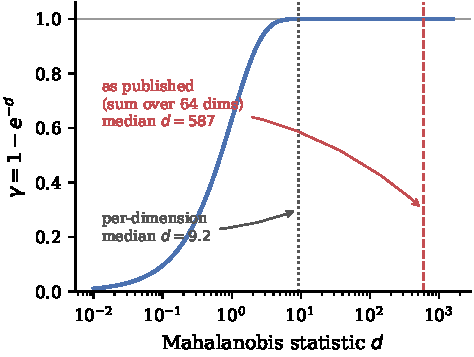
\includegraphics[width=0.92\columnwidth]{fig_saturation.pdf}
\caption{PeTTA's gating function. Because the Mahalanobis statistic is summed over $64$
embedding dimensions, the cross-building median of $587$ sits far inside the saturated
region, giving $\bar\gamma=1$ and an update rate of zero.}
\label{fig:saturation}
\end{figure}

Normalising per dimension unfreezes the mechanism, and it still does not improve on the
source model. An $\alpha$ floor alone does not help, because $\lambda_t=\bar\gamma\lambda_0$
is simultaneously pinned at maximum pull-back. We emphasise that saturation is a failure
mode PeTTA's authors themselves document for ablated variants; what is new here is that it
occurs for the full method when the domain gap is a change of building rather than an
image corruption.

\paragraph{DIGA: published hyperparameters do not transfer.} Table~\ref{tab:diga} crosses
the two readings of DIGA's prototype similarity with two hyperparameter settings.

% source: /tmp/diga_sim.py over tta_faithful.DIGAFaithful
\begin{table*}[t]
\centering
\caption{DIGA under two readings of Eq.~8 and two hyperparameter settings. Source-only is
\macf{} $0.4641$, MCC $0.4679$.}
\label{tab:diga}
\small
\begin{tabular}{llccc}
\toprule
Reading of $\langle\cdot,\cdot\rangle$ & Hyperparameters & Changed & \macf & MCC \\
\midrule
Inner product (literal) & published $0.8/0.9$   & $2573/3412$ & $0.2151$ & $0.1840$ \\
Inner product (literal) & retuned $0.95/0.50$   & $3404/3412$ & $0.0075$ & $-0.1674$ \\
Squared distance        & published $0.8/0.9$   & $1324/3412$ & $0.3932$ & $0.3610$ \\
Squared distance        & retuned $0.95/0.50$   & $357/3412$  & $\mathbf{0.4808}$ & $\mathbf{0.4867}$ \\
Cosine                  & published $0.8/0.9$   & $931/3412$  & $0.3232$ & $0.3399$ \\
Cosine                  & retuned $0.95/0.50$   & $263/3412$  & $0.4750$ & $0.4825$ \\
\bottomrule
\end{tabular}
\end{table*}

The literal inner-product reading yields a negative MCC, confirming that
$\langle\cdot,\cdot\rangle$ must denote a dissimilarity. More substantively, DIGA's
published hyperparameters lose $8.8$ \macf{} points against retuned values on this data.
DIGA's own evaluation makes a point of using a single global parameter set across all
experiments, in explicit contrast to competitors tuned per source--target pair. That
property does not survive the move to one-dimensional sensor data, and recovering the loss
required tuning on target labels, which deployment does not provide.

\subsection{Occupancy estimation}
\label{sec:res-oe}

Table~\ref{tab:oe} runs the identical model and methods under three normalisation
protocols.

% source: results/exp13_occ_scaler.csv (src/exp13_occ_scaler.py), 5 seeds
\begin{table*}[t]
\centering
\caption{Occupancy estimation, MCC on the target test set ($n=150$, $34$ minority), under
three normalisation protocols. Always predicting ``not occupied'' gives MCC $0.000$.}
\label{tab:oe}
\begin{tabular}{lccc}
\toprule
Method & Fitted on source & Fitted on target train & Fitted on target train $+$ test \\
\midrule
Source-only & $\mathbf{0.6583}\pm0.013$ & $\mathbf{0.6951}\pm0.013$ & $\mathbf{0.6966}\pm0.017$ \\
AdaBN       & $0.6412$ & $0.6232$ & $0.6323$ \\
DIGA        & $0.6401$ & $0.6693$ & $0.6769$ \\
PETAL       & $0.6583$ & $0.6951$ & $0.6966$ \\
PeTTA       & $0.6583$ & $0.6951$ & $0.6966$ \\
\bottomrule
\end{tabular}
\end{table*}

Three results follow from Table~\ref{tab:oe}, all of them about the forward direction;
the reverse is taken up below. No method improves on the source model under any of the
three normalisation protocols, and DIGA is below the baseline in all three columns. The choice of normalisation is worth $+3.8$ MCC
points, but it is worth that to \emph{every} method equally, including the unadapted
baseline. It is normalisation, not adaptation, and a protocol that fits the scaler on
target statistics will credit it to whichever method happens to be under test. Finally,
PETAL and PeTTA reproduce
source-only predictions to four decimal places on this task as well, which rules out a
HAR-specific explanation for the two freezes reported in Section~\ref{sec:res-mech}.

Running the transfer in the reverse direction --- training on the target office and
evaluating on the source office --- changes the picture completely, and in a way that is
the most direct evidence in this paper for its central claim.

% source: results/exp17_occ_reverse.csv (src/exp17_occ_reverse.py), 5 seeds
\begin{table*}[t]
\centering
\caption{Occupancy in both transfer directions, MCC, source-fitted normalisation, 5 seeds.
The only thing that differs between the two columns is which office supplies the source
model. Always predicting ``not occupied'' gives MCC $0.000$ in both.}
\label{tab:oe-rev}
\small
\begin{tabular}{lcc}
\toprule
Method & source $\to$ target & target $\to$ source \\
\midrule
Source-only & $\mathbf{0.6583}$ & $-0.0775$ \\
AdaBN       & $0.6412$ & $\mathbf{0.3374}$ \\
DIGA        & $0.6401$ & $0.1934$ \\
PETAL       & $0.6583$ & $-0.0775$ \\
PeTTA       & $0.6583$ & $-0.0775$ \\
\bottomrule
\end{tabular}
\end{table*}

In the reverse direction the source checkpoint is not merely weak but worse than chance:
trained on the target office, it reaches MCC $-0.0775$ on the source office, meaning its
predictions are anti-correlated with the labels. Against that starting point AdaBN
improves MCC by $41.5$ points and DIGA by $27.1$. In the forward direction, starting from
a checkpoint at $0.6583$, the same two methods lose $1.7$ and $1.8$ points respectively.

The contrast is as clean as this dataset allows: identical methods, identical protocol,
identical features, two offices, and the only variable is whether the source model was any
good. When it is, adaptation has nothing to contribute and the normalisation-based methods
actively harm it; when it is broken, the same methods recover a large part of the deficit.
This mirrors AdaBN's behaviour on HAR, where it costs $17$ \macf{} points against a sound
checkpoint, and it supports reading adaptation gain as a measure of source-model
deficiency rather than of adaptation quality. A method evaluated only against a weak
source model will appear to work.

PETAL and PeTTA reproduce the source predictions exactly in this direction too. Across two
tasks and two directions each, neither method has changed a prediction.

% ============================================================================
\section{Discussion}
\label{sec:discussion}

The headline result of this study is not about any one method. It is that the quantity
these methods are asked to repair --- the cross-building performance drop --- was being
measured in a way that substantially overstated it, and that most of what remains after
correcting the measurement is attributable to feature design rather than to anything TTA
can reach.

Measured consistently on both sides, the gap is $9$ to $15$ points of \macf{} depending on
direction, against the $83$ points implied by comparing a leakage-inflated source figure
with an honest target one. A model built from thirteen layout-invariant statistics
transfers to a different apartment at close to its own in-domain ceiling. That ceiling, in
turn, becomes the binding constraint: one cannot improve target performance much beyond
source performance, which is why our attempts to push the source model further --- richer
invariant features, class weighting, wider networks --- gained little. Only causal
smoothing helped, and modestly.

The recurrence of the inversion is what we would most want a reader to take away.
It appears when choosing features (a set validating at $0.623$ transfers at $0.300$, while
one validating at $0.534$ transfers at $0.447$), when choosing window length ($0.5611$
in-domain at $W{=}60$ against $0.4260$ on the target), when adding temporal context (the
TCN validates at $0.5414$ and transfers at $0.4082$), and in the reverse direction, where
the conventional $135$-d vector records the best source-validation score of any
configuration in this study and the worst transfer, below chance. Five instances, four
different design decisions, both directions.

A single mechanism accounts for all of them. Every one of these choices increases the
model's access to building-specific regularity: which device fired, what the routine looks
like over an hour, how this occupant sequences their morning. In-domain that is signal.
Across buildings it is noise with the wrong sign. The practical consequence, stated with the scope
it has earned: in this data, for cross-building deployment, in-domain validation accuracy
was not merely an imperfect model-selection criterion but an actively misleading one.
Whether that holds beyond these two apartments is open, and Section~\ref{sec:discussion}
returns to what would settle it.

This reframes what per-sensor features cost. In-domain they are valuable: the best
source-validation score in Table~\ref{tab:features} belongs to a set that retains them.
Across buildings they are worse than useless, scoring below chance alone in both
directions. The inversion between in-domain fit and cross-building transfer is, we think,
the most portable finding here, and it has a practical consequence: model selection on
in-domain validation will systematically choose the configuration that transfers worst.
Practitioners selecting a source checkpoint for cross-building deployment should not use
in-domain accuracy to do it.

On the methods themselves, the three failures are instructive precisely because they are
different from one another. PETAL's is a reading failure with a sharp edge: a coefficient
that looks like a regulariser weight scales the likelihood, and the hyperparameter search
most practitioners would run --- selecting on target performance --- actively prefers the
value that disables adaptation. PeTTA's is dimensional: a divergence statistic that behaves
sensibly when the domain gap is a corruption of the same image saturates when the gap is a
different building, and because the mechanism fails silently the loss curves look
unremarkable throughout. DIGA's is about generality: it works, but the single global
parameter set it advertises does not, and the gap between its published and retuned
settings is larger than the gain adaptation produces.

A practical consequence runs through all three. Hyperparameter selection on held-out target
labels, which is standard in this literature, is not merely optimistic. It can select degenerate configurations, as the PETAL sweep shows, and it can
make a method appear to transfer when what transferred was the tuning. A label-free
criterion should be reported alongside any oracle-tuned number.

The occupancy results in both directions (Table~\ref{tab:oe-rev}) are the cleanest
demonstration of this available here, because they hold everything constant but the
quality of the source model. Starting from a checkpoint at MCC $0.658$, adaptation costs
roughly two points; starting from one at $-0.078$, the same methods gain twenty-seven to
forty-one. The methods did not change. What changed is how much room there was.

\paragraph{What generalises, and what does not.} The findings above differ in how far
they travel, and it is worth separating them.

Two do not depend on this dataset at all. PETAL's $\bar\lambda$ multiplies the
cross-entropy in its published objective (Eq.~\ref{eq:petal}), so $\bar\lambda=0$ removes
the data term on any dataset, in any modality; the only dataset-specific part of our
result is that tuning on target labels happened to select it. PeTTA's gating function
likewise saturates whenever the summed Mahalanobis statistic is large, which is a property
of summing over embedding dimensions rather than of these apartments --- though whether
the statistic reaches that regime does depend on how far apart the domains are, and the
authors' own traces on image corruptions sit at $0.8$--$1.0$ rather than at unity.

The evaluation result is a property of a procedure rather than of a dataset: stride-$1$
windowing with a random validation split places near-duplicates across the split whenever
windows overlap, which is common in sensor-based HAR.

The inversion is different in kind. We observe it five times across four design decisions
and in both transfer directions, which rules out a one-off, but all five observations come
from the same two apartments. We therefore state it as an empirical regularity of this
data rather than as a general law: \emph{in this dataset, across every design choice we
varied, the configuration selected by in-domain validation was the one that transferred
worst.} If it holds more widely it inverts standard model-selection practice for
cross-building deployment, and we think the mechanism --- that each of these choices
increases access to building-specific regularity --- is general enough to be worth
testing elsewhere. Establishing that requires datasets with more than two environments.

\paragraph{Limitations.} The study rests on one HAR dataset and two apartments from it.
Running both transfer directions rules out a direction-specific fluke but says nothing
about other buildings, other sensor modalities, or richer activity sets; external validity
beyond these two apartments is untested, and the dataset contains no further homes. The
occupancy data is private, so that section is not independently
reproducible from the released code. Our best configuration improves on the simpler one by
$3.3$ \macf{} points against a between-fold standard deviation of $0.067$, and we present
it as a modest gain rather than a result. And the \texttt{cleaning} class, with $113$ target
samples, is not learned by any method we tried; whether that is a sample-size limit or a
representational one, we cannot say from these data.

% ============================================================================
\section{Conclusion}
\label{sec:conclusion}

We evaluated three image-domain test-time adaptation methods on cross-building human
activity recognition and occupancy estimation, and found that the evaluation protocol
dominated the comparison. Stride-one windowing with a random validation split inflates
source-domain \macf{} from roughly $0.53$ to $0.998$; grouping the split by recording day
removes the effect, and the window definition is nearly irrelevant to it. Making features
causal, which the online premise of TTA requires, improves target transfer by $7.3$ points
rather than costing anything.

Across every design choice we varied --- feature set, window length, temporal context ---
and in both transfer directions, the configuration that validated best in-domain
transferred worst. Five observations on two apartments do not establish a general law, but
they do establish that in-domain validation cannot be assumed safe for cross-building
model selection. Under the grouped protocol the cross-building gap is $9$ to $15$ points depending on
direction, and most of it is attributable to features that encode sensor identity. Those
features score below stratified-random guessing on the target in both directions. The
feature set that validates best in-domain transfers worst, also in both directions.

Of the three methods, only DIGA improves on this baseline, by $1.7$ \macf{} points
with a bootstrap interval excluding zero, and only with hyperparameters retuned on target
labels. PETAL and PeTTA do not adapt at all, for reasons traceable to specific equations:
PETAL's coefficient scales the likelihood, so the value selected by target-label tuning
removes the learning signal; PeTTA's divergence signal sums over the embedding dimension
and saturates when the domains are buildings. Both failures reproduce on occupancy
estimation, in both of its transfer directions. Occupancy also isolates what an adaptation
gain measures: the two directions differ only in the quality of the source checkpoint, and
against a sound one no method improves, while against one that is worse than chance the
same methods gain $27$ to $41$ MCC points. A further apparent gain proves attributable to
a target-fitted normalisation worth $3.8$ MCC points to every method, the unadapted one
included.

We do not conclude that test-time adaptation is unsuitable for smart buildings. We conclude
that it was being asked to repair a problem largely created by evaluation and feature
design, and that fixing those leaves little for adaptation to contribute. Future work
should look at making building-specific information transferable rather than discarding
it --- aligning sensors across sites by functional role, using unlabelled co-activation
structure --- since the $9$ points separating our layout-invariant features from the
best in-domain configuration are exactly the information currently being thrown away.

% ============================================================================
\section*{Reproducibility}

Code, the raw sensor data and every result file are available at
\url{https://github.com/TCVHN5Vn/TTA-Test-Time-Adaptation}. The repository reproduces the
full analysis from the raw CSVs in one pass, each table above names the script and result
file that generated it. The occupancy dataset is private --- it
was collected at the Grenoble Institute of Technology and is not ours to redistribute ---
so that section alone is reported but not independently reproducible. Implementations of
the three adaptation methods as originally applied are at
\url{https://github.com/TCVHN5Vn/Test-Time-Adaptation}.

\section*{Acknowledgements}

This research was supported by the Natural Sciences and Engineering Research Council of
Canada (NSERC).

% ============================================================================
\appendix
\section{A larger layout-invariant feature set}
\label{app:inv}

We also evaluated a $60$-dimensional invariant set adding a sorted activation profile (the
per-sensor window means sorted in descending order, which is invariant to any permutation
of sensor indices), run-length and recency structure, and the window statistics recomputed
at $W\in\{5,10,40\}$. It does not help:

\begin{table*}[t]
\centering
\caption{Richer layout-invariant features, S1$\to$S2, GroupKFold, 3 seeds.}
\begin{tabular}{lcc}
\toprule
Feature set & $d$ & Target \macf \\
\midrule
Global $+$ temporal                      & 13 & $\mathbf{0.4350}\pm0.061$ \\
$+$ sorted activation profile            & 28 & $0.4245\pm0.039$ \\
$+$ run-length structure                 & 33 & $0.4227\pm0.027$ \\
$+$ multi-scale windows                  & 60 & $0.4188\pm0.028$ \\
\bottomrule
\end{tabular}
\end{table*}

Permutation invariance in sensor index is evidently not sufficient: S1 has $70$ sensors and
S2 has $75$, placed in differently shaped rooms, so ``how many sensors are busy and how
concentrated the activity is'' is itself building-specific. Inverse-frequency class
weighting also failed, reducing \macf{} to $0.3852$ and \emph{lowering} balanced accuracy
from $0.4818$ to $0.4280$, most plausibly because it pushes the model toward
\texttt{cleaning}, which is not learnable from $113$ target samples, at the cost of the
four classes that do work.

% ============================================================================
\begin{thebibliography}{99}

\bibitem{manfren2021} M. Manfren, M. Sibilla, L. Tronchin, Energy modelling and analytics
in the built environment---a review of their role for energy transitions in the
construction sector, Energies 14 (3) (2021) 679.

\bibitem{amangeldy2025} B. Amangeldy, T. Imankulov, N. Tasmurzayev, G. Dikhanbayeva,
Y. Nurakhov, A review of artificial intelligence and deep learning approaches for resource
management in smart buildings, Buildings 15 (15) (2025) 2631.

\bibitem{dridi2022} J. Dridi, M. Amayri, N. Bouguila, Transfer learning for estimating
occupancy and recognizing activities in smart buildings, Building and Environment 217
(2022) 109057.

\bibitem{amayri2019} M. Amayri, S. Ploix, N. Bouguila, F. Wurtz, Estimating occupancy using
interactive learning with a sensor environment: real-time experiments, IEEE Access 7 (2019)
53932--53944.

\bibitem{dridi_cluster} J. Dridi, M. Amayri, N. Bouguila, Unsupervised clustering-based
domain adaptation for estimating occupancy and recognizing activities in smart buildings,
Journal of Building Engineering 85 (2024) 108741.

\bibitem{shahbazian2023} R. Shahbazian, I. Trubitsyna, Human sensing by using radio
frequency signals: a survey on occupancy and activity detection, IEEE Access 11 (2023)
40878--40904.

\bibitem{hong2017} T. Hong, D. Yan, S. D'Oca, C. Chen, Ten questions concerning occupant
behavior in buildings: the big picture, Building and Environment 114 (2017) 518--530.

\bibitem{liang2024} J. Liang, R. He, T. Tan, A comprehensive survey on test-time adaptation
under distribution shifts, International Journal of Computer Vision 133 (1) (2025) 31--64.

\bibitem{diga} W. Wang, Z. Zhong, W. Wang, X. Chen, C. Ling, B. Wang, N. Sebe, Dynamically
instance-guided adaptation: a backward-free approach for test-time domain adaptive semantic
segmentation, in: CVPR, 2023, pp. 24090--24099.

\bibitem{petal} D. Brahma, P. Rai, A probabilistic framework for lifelong test-time
adaptation, in: CVPR, 2023, pp. 3582--3591.

\bibitem{petta} T.-H. Hoang, D. M. Vo, M. N. Do, Persistent test-time adaptation in
recurring testing scenarios, in: NeurIPS, Vol. 37, 2024.

\bibitem{tent} D. Wang, E. Shelhamer, S. Liu, B. Olshausen, T. Darrell, Tent: fully
test-time adaptation by entropy minimization, in: ICLR, 2021.

\bibitem{cotta} Q. Wang, O. Fink, L. Van Gool, D. Dai, Continual test-time domain
adaptation, in: CVPR, 2022, pp. 7201--7211.

\bibitem{shot} J. Liang, D. Hu, J. Feng, Do we really need to access the source data?
Source hypothesis transfer for unsupervised domain adaptation, in: ICML, Vol. 119 of PMLR,
2020, pp. 6028--6039.

\bibitem{abderrahim2025} O. Abderrahim, J. Dridi, M. Amayri, N. Bouguila, Occupancy
estimation and activity recognition in smart buildings using open set domain adaptation,
Journal of Building Engineering 112 (2025) 113784.

\bibitem{abderrahim2026} O. Abderrahim, J. Dridi, M. Amayri, N. Bouguila, Scalable activity
recognition in smart buildings via generalized domain adaptation of IoT sensor data, Energy
and Buildings 351 (2026) 116692.

\bibitem{abderrahim_osda} O. Abderrahim, J. Dridi, M. Amayri, N. Bouguila, Open set domain
adaptation and universal domain adaptation for enhancing activity recognition in smart
buildings, in: Proceedings of the 19th IBPSA Conference, Brisbane, Australia, 2025.
\url{https://doi.org/10.26868/25222708.2025.1331}.

\bibitem{wang2023} S. Wang, J. Wang, H. Xi, B. Zhang, L. Zhang, H. Wei, Optimization-free
test-time adaptation for cross-person activity recognition, Proceedings of the ACM on
Interactive, Mobile, Wearable and Ubiquitous Technologies 7 (4) (2023) 183.

\bibitem{tapia2004} E. M. Tapia, S. S. Intille, K. Larson, Activity recognition in the
home using simple and ubiquitous sensors, in: Pervasive Computing, Springer, Berlin,
Heidelberg, 2004, pp. 158--175.

\bibitem{chicco2020} D. Chicco, G. Jurman, The advantages of the Matthews correlation
coefficient (MCC) over F1 score and accuracy in binary classification evaluation, BMC
Genomics 21 (1) (2020) 6.

\end{thebibliography}

\end{document}
